\documentclass[bachelor, och, labwork]{shiza}

\usepackage[utf8]{inputenc}
\usepackage{graphicx}

\usepackage[table,xcdraw]{xcolor}

\usepackage[sort,compress]{cite}
\usepackage{amsmath}
\usepackage{amssymb}
\usepackage{amsthm}
\usepackage{fancyvrb}
\usepackage{longtable}
\usepackage{array}
\usepackage[english,russian]{babel}
\usepackage{minted}

\usepackage{tempora}

% \usepackage{xcolor,colortbl}
% \definecolor{pink}{HTML}{FF9B9B}
% \newcommand{\done}{\cellcolor{teal}done}  %{0.9}
% \newcommand{\hcyan}[1]{{\color{teal} #1}}

% \usepackage[colorlinks=false]{hyperref}


\newcommand{\eqdef}{\stackrel {\rm def}{=}}

\newcommand{\specialcell}[2][c]{%
  \begin{tabular}[#1]{@{}c@{}}#2\end{tabular}}

\begin{document}

\title{Алгоритмы алгебры и теории чисел}

\course{4}

\group{431}

\napravlenie{10.05.01 "--- Компьютерная безопасность}


\author{Никитина Арсения Владимировича}


\satitle{доцент}
\saname{А.\,С.\,Гераськин}


\date{2022}

\maketitle

% Включение нумерации рисунков, формул и таблиц по разделам
% (по умолчанию - нумерация сквозная)
% (допускается оба вида нумерации)
%\secNumbering


\tableofcontents

\section{Задание лабораторной работы}

Вычисление значений и корней полиномов.

\section{Теоретическая часть}

В данной работе будет рассмотрен алгоритм нахождения корней и значений полиномов
с помощью схемы Горнера.


Теорема Безу, несмотря на внешнюю простоту и очевидность, является одной из 
фундаментальных теорем теории многочленов. В этой теореме алгебраические свойства 
многочленов (которые позволяют работать с многочленами как с целыми числами) 
связываются с их функциональными свойствами (которые позволяют рассматривать 
многочлены как функции).


\begin{center}
    \textit{Теорема Безу}
\end{center}

Остаток от деления многочлена  $F(x)$  на линейный двучлен  $x-a$  равен 
значению многочлена в точке $a$, т.е. числу $F(a)$.

\underline{Доказательство}

Поделим с остатком многочлен $P(x)$ на двучлен $x-a$:

$P(x)=(x-a)Q(x)+R(x)$, где $R(x)$ --- остаток. Так как $\deg R(x)<\deg(x-a)=1$,
то $R(x)$ --- многочлен степени не выше 0, то есть константа, обозначим её за 
$r$. Подставляя $x=a$, поскольку $(a-a)Q(a)=0$, имеем $P(a)=R(x)=r$.

\underline{Следствия}

\begin{enumerate}
    \item Число $a$ является корнем многочлена $p(x)$ тогда и только тогда, 
    когда $p(x)$ делится без остатка на двучлен $x-a$ (отсюда, в частности, 
    следует, что множество корней многочлена $P(x)$ тождественно множеству корней
    соответствующего уравнения $P(x)=0$).
    \item Свободный член многочлена делится на любой целый корень многочлена с 
    целыми коэффициентами (если старший коэффициент равен 1, то все рациональные 
    корни являются и целыми).
    \item Пусть $a$ --- целый корень приведённого многочлена $A(x)$ с целыми 
    коэффициентами. Тогда для любого целого $k$ число $A(k)$ кратно $a-k$.
\end{enumerate}

Схема Горнера --- алгоритм деления многочленов, записанный для частного случая, 
когда частное равно двучлену $x-a$.

\begin{center}
    \textit{Схема Горнера}
\end{center}

Пусть $P(x)=a_nx^n + a_{n-1}x^{n-1}+ \dotsc + a_0$ --- делимое,
$Q(x)=b_{n-1}x^{n-1}+b_{n-2}x^{n-2}+\dotsc+b_0$ --- частное (его степень,
очевидно, будет на 1 меньше), $r$ --- остаток (так как деление осуществляется на
многочлен 1-ой степени, то степень остатка будет на 1 меньш, то есть нулевая,
значит, остаток --- константа).

По определению деления с остатком $P(x) = Q(x) \cdot (x-a) + r$.

После подстановки выражений многочленов получим: 

$a_nx^n + a_{n-1}x^{n-1} + a_0 = \left( b_{n-1}x^{n-1} + b_{n-2}x^{n-2} + \dotsc b_0\right) \cdot (x-a) + r.$

Раскроем скобки и приравняем коэффициенты при одинаковых степенях, после чего 
легко выразить коэффициенты частного через коэффициенты делимого и делителя.

\begin{table}[htb]
    \centering
    \begin{tabular}{|l|l|lll}
        \cline{1-2}
        \specialcell{Коэффициенты при \\одинаковых степенях} & \specialcell{Выражение коэффициентов $b_k$ \\через коэффициенты $a_k$} &  &  &  \\ \cline{1-2}
        $a_n=b_{n-1}$                        & $b_{n-1}=a_n$                                          &  &  &  \\ \cline{1-2}
        $a_{n-1}=b_{n-1} - ab_{n-1}$         & $b_{n-2}=ab_{n-1}+a_{n-1}$                              &  &  &  \\ \cline{1-2}
        $\cdots$                             & $\cdots$                                               &  &  &  \\ \cline{1-2}
        $a_k=b_{k-1} - ab_k$                 & $b_{k-1}=a_k + ab_k$                                   &  &  &  \\ \cline{1-2}
        $\cdots$                             & $\cdots$                                               &  &  &  \\ \cline{1-2}
        $a_0=r-ab_0$                         & $r=ab_0+a_0$                                           &  &  &  \\ \cline{1-2}
    \end{tabular}
\end{table}

Затем вычисления сводятся в следующую таблицу:

\begin{table}[hbt]
    \centering
    \begin{tabular}{l|l|l|l|
    >{\columncolor[HTML]{FF9B9B}}l |l|l|}
    \hline
    \multicolumn{1}{|l|}{\cellcolor[HTML]{FF9B9B}$a$} & $a_n$         & $\cdots$ & $\cdots$                      & $a_k$                 & $\cdots$ & $a_0$        \\ \hline
                                                      & $b_{n-1}=a_n$ & $\cdots$ & \cellcolor[HTML]{FF9B9B}$b_k$ & $b_{k-1}=a_k + a b_k$ & $\cdots$ & $r=ab_0+a_0$ \\ \cline{2-7} 
    \end{tabular}
    \end{table}


В таблице выделены те клетки, содержимое которых участвует в вычислениях на 
очередном шаге.

В алгоритме нахождения значений полинома в точке в с помощью результата работы
алгоритма нахождения разложения полинома по теореме Горнера находится требуемое
значение.

\section{Практическая часть}
\subsection{Пример работы алгоритма}
\begin{figure}[H]
    \centering
    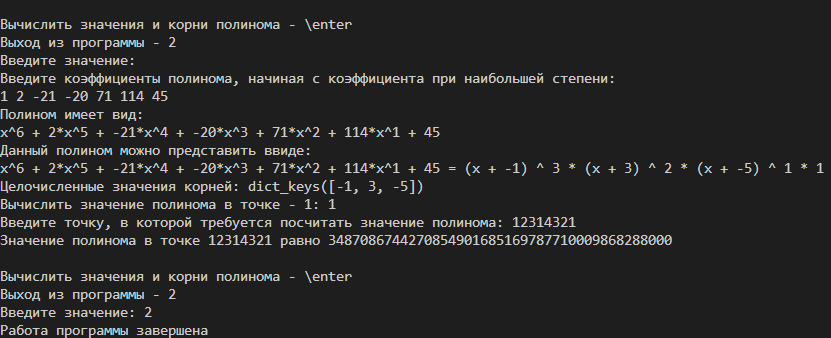
\includegraphics[width=1\textwidth]{pic1.png}
    \caption{}
\end{figure}

\setminted[python]{linenos,breaklines=true, fontsize=\small, style=bw}
    \subsection{Код программы, реализующей рассмотренный алгоритм}
        \inputminted{python}{lab15.py}


\end{document}